\documentclass[diploma]{BMSTU-IU8}

\usepackage{todonotes}
\usepackage{lipsum}
\SetLipsumText{fishes}

\student{И. И. Иванов}
\theme{Создание отчёта \\ по НИРС \\ или ВКР}
\group{ИУ8-999}

\supervisor{П. П. Петров}
\researchConsultant{П. П. Петров}
\designConsultant{П. П. Петров}
\technologicalConsultant{П. П. Петров}
\economicsConsultant{П. П. Петров}
\lawsConsultant{П. П. Петров}
\normController{П. П. Петров}

% \theme{Тест \hfill} % Тема для НИРСа заполняется по-другому
\studentFullName{Иванов Иван Иванович}
\profile{10У101}
\speciality{10.05.01 <<Компьютерная безопасность>>}
\specialization{10.05.01\_01 <<Математические методы защиты информации>>}
\supervisorWithDegree{доцент, к.т.н. Иванов И. И.}

\newglossaryentry{id1}{ % Нужны разные id, можно ставить просто последовательно
        name={\LaTeX},
        description={система компьютерной вёрстки} 
}
\newglossaryentry{id2}{
        name={МГТУ},
        description={Московский государственный технический университет} 
}
\newglossaryentry{id3}{
        name={$S^{2}$},
        description={Формула в списке обозначений} 
}
\newglossaryentry{id1}{ % Нужны разные id, можно ставить просто последовательно
    name={\LaTeX},
    description={система компьютерной вёрстки} 
}
\newglossaryentry{id2}{
    name={МГТУ},
    description={Московский государственный технический университет} 
}
\newglossaryentry{id3}{
    name={$S^{2}$},
    description={формула в списке обозначений} 
}


\addbibresource{main.bib}
    
\begin{document}
    \maketitle
    % % \inlineimg{example.png}{\img}
    % \maketitle % Титульный лист

    % % 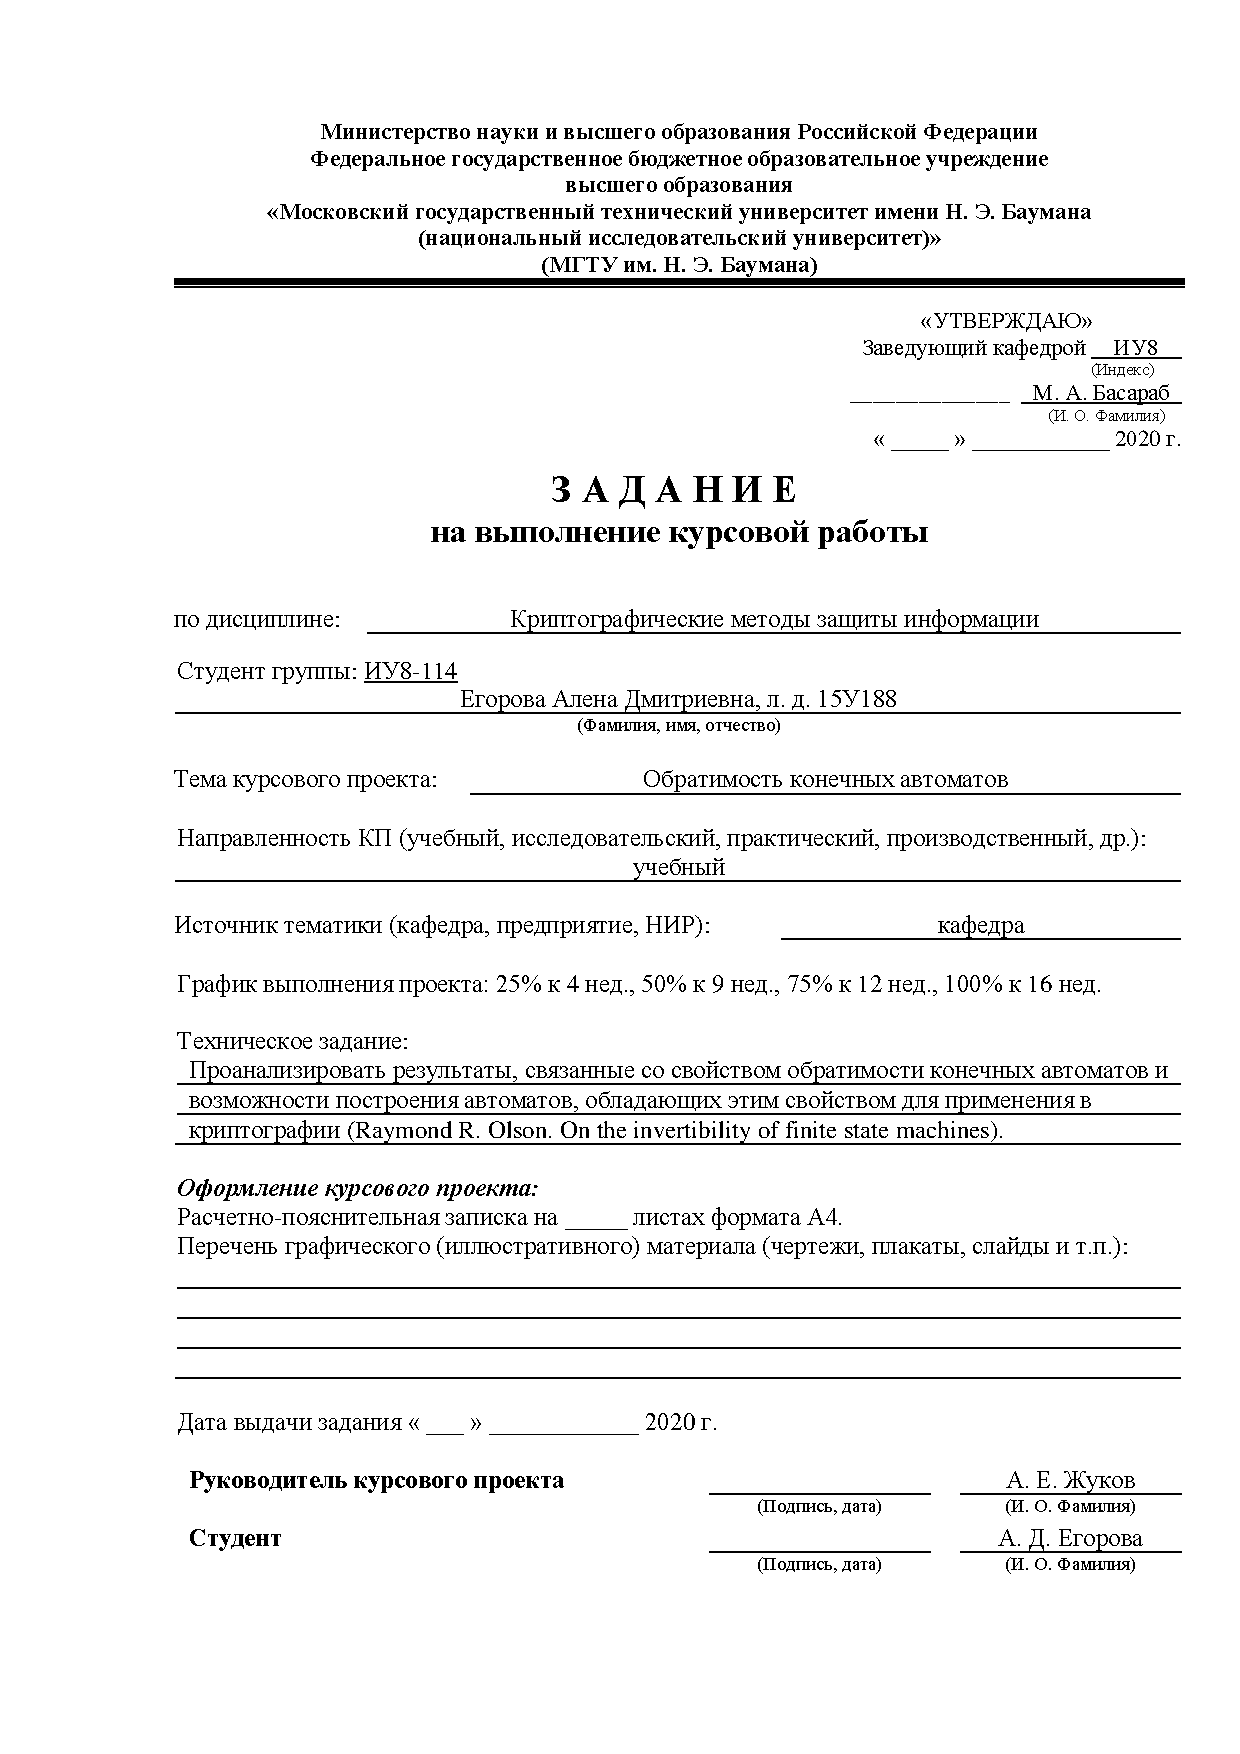
\includepdf[pages=-]{extra/task} % Задание
    % % \setcounter{page}{3} % Устанавливает счётчик страниц

    \abstract % Структурный элемент: РЕФЕРАТ

\lipsum[1-2]
 % Реферат

    \tableofcontents % Содержание 
    \termsanddefenitions % Термины и определения
    \listofabbreviations % Перечень сокращений и обозначений
 
    \introduction % Структурный элемент: ВВЕДЕНИЕ

\lipsum[1-5]

Цитирование источника 1 \cite{Wikipedia1}.
 % Введение

    \section{Использование титульной страницы}

Для того, чтобы подключить нужную титульную страницу, необходимо 
указать параметр \texttt{diploma} или \texttt{research} в классе документа. 
Это НИРС или ВКР соответственно. 

Заполнение полей показано в файле \texttt{main.tex}, приведу ещё раз здесь. 
Желательно заполнить все поля по образцу, чтобы не было проблем с тем, 
что что-то может быть не определено.

\begin{verbatim}
\theme{Создание отчёта по НИРС или курсовой}
\group{ИУ8-999}
\profile{10У101}
\speciality{10.05.01 <<Компьютерная безопасность>>}
...
\end{verbatim}

\lipsum[1-5]

Цитирование источника 2 \cite{Wikipedia2}.

    \section{Техническое задание и календарный план}

Эти части слишком вариативны, так что сделайте их либо самостоятельно, либо в Ворде, а затем вклейте. Не забудьте поменять счётчик листов.
    \section{Создание реферата}

Первая строка там уже есть --- с использованием счётчиков страниц, рисунков, 
таблиц, источников и приложений. 
Необходимо заполнить ключевые слова и краткий обзор своей работы, 
куда входит цель, этапы и прочее...

\lipsum[1-4]

Цитирование источника 4 \cite{Wikipedia4} \cite{cite_1_2} \cite{cite_1_15} \cite{cite_1_16}.

    \section{Задание списка терминов, сокращений и определений}

Насколько я понимаю, этим заниматься особо никто не любит и, если и делает, 
то для того, чтобы он был, вставляя туда по три-четыре определения. 
Специально для того, чтобы можно было создать этот список, есть файл 
\texttt{glossary.tex}, который подключается до начала документа. 
В нём по заданному образцу нужно записать те обозначения и сокращения, 
которые вы хотели бы видеть в своей работе. 

Для того чтобы этот список подключился в качестве части отчёта/РПЗ, 
нужно использовать команду \texttt{\textbackslash glossaries}. В этом 
шаблоне она идёт сразу после \texttt{\textbackslash tableofcontents}, так 
что можете либо оставить её, заполнив своими терминами соответствующий файл, 
либо просто удалить/закомментировать команду.

    \section{Использование рисунков}

Вставляются рисунки как обычно --- через \texttt{\textbackslash includegraphics} и окружение \texttt{figure}. Пожалуйста, не используйте \texttt{[H]} --- в этом шаблоне уже настроена среда картинок так, что она вставится как можно ближе к тексту по возможности. Использование \texttt{[H]} приводит к большим и некрасивым разрывам текста. Это же касается и таблиц.

На рисунке~\ref{fig:fig01} показан герб МГТУ. Также тут видно, что ссылка на рисунок работает.

\begin{figure}
  \centering
  
\includegraphics[scale=0.7]{inc/bmstu}
  \caption{Герб МГТУ}
  \label{fig:fig01}
\end{figure}

% \subsection{Две картинки в одной (subcaption)}

% Выше видно как работает задание подраздела. 

% Также можно делать два рисунка в одном, чтобы подписать их, например, как рисунок~\ref{} и рисунок~\ref{}.


    \section{Цитирование источников}

Вот так \cite{Article} можно цитировать статьи. 
Заполнение представлено в файле \texttt{main.bib}. 
Пожалуйста, указывайте \texttt{russian} в качестве параметра \texttt{language}!

Аналогично можно цитировать сайты в интернете, но нужно будет добавить 
дату обращения \cite{Wikipedia}.

Также можно вставлять ссылки командой \url{https://vk.com}, например.

Больше примеров для оформления библиотграфических ссылок можно найти в 
документации к пакету \texttt{gost2008}: 
\url{http://tug.ctan.org/tex-archive/biblio/bibtex/contrib/gost/doc/examples/cp1251/gost2008.pdf}.



\lipsum[1-4]

Цитирование источника 2 \cite{cite_1_11}.

    \section{Работа с таблицами}

Далее рассматриваются варианты создания таблиц. На этом моменте лучше смотреть в исходник.

\subsection{Использование tabular}

Самый простой и стандартный способ --- использование tabular. Так мы создали таблицу~\ref{tab:tab1}. Обратите внимание на использование \texttt{hhline} --- этот пакет позволяет подчёркивать не всю линию, а только те столбцы, которые нужно подчеркнуть. Полезно при использовании мультистрок или мультистолбцов.

\begin{table}    
    \caption{Пример короткой таблицы с использованием tabular}
    \begin{tabular}{|r|c|c|c|l|}\hline
    Тело      & $F$ & $V$  & $E$ & $F+V-E-2$ \\ \hline
    Тетраэдр  & 4   & 4    & 6   & 0         \\ \hhline{~-~-~}
    Куб       & 6   & 8    & 12  & 0         \\ \hhline{--~~~}
    Октаэдр   & 8   & 6    & 12  & 0         \\ \hhline{-----}
    Додекаэдр & 20  & 12   & 30  & 0         \\ \hline
    Икосаэдр  & 12  & 20   & 30  & 0         \\ \hline
    \end{tabular}
    \label{tab:tab1}
\end{table}

\subsection{Использование tabularx}

Этот способ мне нравится больше, потому что позволяет задать ширину таблицы~\ref{tab:tab2}. Единственное ограничение --- в этой таблице должен быть столбец, обозначаемый \texttt{X}, который может быть растянут до нужного размера (заполнения листа).

\begin{table}    
    \caption{Пример короткой таблицы с tabularx}
    \begin{tabularx}{\textwidth}{|X|c|c|c|l|}\hline
    Тело      & $F$ & $V$  & $E$ & $F+V-E-2$ \\ \hline
    Тетраэдр  & 4   & 4    & 6   & 0         \\ \hhline{~-~-~}
    Куб       & 6   & 8    & 12  & 0         \\ \hhline{--~~~}
    Октаэдр   & 8   & 6    & 12  & 0         \\ \hhline{-----}
    Додекаэдр & 20  & 12   & 30  & 0         \\ \hline
    Икосаэдр  & 12  & 20   & 30  & 0         \\ \hline
    \end{tabularx}
    \label{tab:tab2}
\end{table}

\subsection{Использование longtable}

\texttt{longtable} используется для задания многостраничных длинных таблиц. Необходимо указать надпись, которая будет над таблицей на следующем листе. Пример ниже, в таблице~\ref{tab:tab3}. Обратите внимание --- здесь уже не нужно использовать среду \texttt{table}.

 
\begin{longtable}[H]{|c|c|c|c|c|}
    \caption{Пример использования длинной таблицы на несколько листов, а также пример использования длинного заголовка таблицы}\label{tab:tab3}\\ \hline
    \endfirsthead
    \caption*{Продолжение таблицы \ref{tab:tab3}}\\ \hline
    \endhead
    \hline
    \endfoot
    \hline
    \endlastfoot
    Тело      & $F$ & $V$  & $E$ & $F+V-E-2$ \\ \hline
    Тетраэдр  & 4   & 4    & 6   & 0         \\ \hhline{~-~-~}
    Куб       & 6   & 8    & 12  & 0         \\ \hhline{--~~~}
    Октаэдр   & 8   & 6    & 12  & 0         \\ \hhline{-----}
    Додекаэдр & 20  & 12   & 30  & 0         \\ \hline
    Икосаэдр  & 12  & 20   & 30  & 0         \\ \hline
    Тело      & $F$ & $V$  & $E$ & $F+V-E-2$ \\ \hline
    Тетраэдр  & 4   & 4    & 6   & 0         \\ \hhline{~-~-~}
    Куб       & 6   & 8    & 12  & 0         \\ \hhline{--~~~}
    Октаэдр   & 8   & 6    & 12  & 0         \\ \hhline{-----}
    Додекаэдр & 20  & 12   & 30  & 0         \\ \hline
    Икосаэдр  & 12  & 20   & 30  & 0         \\ \hline
    Тело      & $F$ & $V$  & $E$ & $F+V-E-2$ \\ \hline
    Тетраэдр  & 4   & 4    & 6   & 0         \\ \hhline{~-~-~}
    Куб       & 6   & 8    & 12  & 0         \\ \hhline{--~~~}
    Октаэдр   & 8   & 6    & 12  & 0         \\ \hhline{-----}
    Додекаэдр & 20  & 12   & 30  & 0         \\ \hline
    Икосаэдр  & 12  & 20   & 30  & 0         \\ \hline
    Тело      & $F$ & $V$  & $E$ & $F+V-E-2$ \\ \hline
    Тетраэдр  & 4   & 4    & 6   & 0         \\ \hhline{~-~-~}
    Куб       & 6   & 8    & 12  & 0         \\ \hhline{--~~~}
    Октаэдр   & 8   & 6    & 12  & 0         \\ \hhline{-----}
    Додекаэдр & 20  & 12   & 30  & 0         \\ \hline
    Икосаэдр  & 12  & 20   & 30  & 0         \\ \hline
    Тело      & $F$ & $V$  & $E$ & $F+V-E-2$ \\ \hline
    Тетраэдр  & 4   & 4    & 6   & 0         \\ \hhline{~-~-~}
    Куб       & 6   & 8    & 12  & 0         \\ \hhline{--~~~}
    Октаэдр   & 8   & 6    & 12  & 0         \\ \hhline{-----}
    Додекаэдр & 20  & 12   & 30  & 0         \\ \hline
    Икосаэдр  & 12  & 20   & 30  & 0         \\ \hline
    Тело      & $F$ & $V$  & $E$ & $F+V-E-2$ \\ \hline
    Тетраэдр  & 4   & 4    & 6   & 0         \\ \hhline{~-~-~}
    Куб       & 6   & 8    & 12  & 0         \\ \hhline{--~~~}
    Октаэдр   & 8   & 6    & 12  & 0         \\ \hhline{-----}
    Додекаэдр & 20  & 12   & 30  & 0         \\ \hline
    Икосаэдр  & 12  & 20   & 30  & 0         \\ \hline
    Тело      & $F$ & $V$  & $E$ & $F+V-E-2$ \\ \hline
    Тетраэдр  & 4   & 4    & 6   & 0         \\ \hhline{~-~-~}
    Куб       & 6   & 8    & 12  & 0         \\ \hhline{--~~~}
    Октаэдр   & 8   & 6    & 12  & 0         \\ \hhline{-----}
    Додекаэдр & 20  & 12   & 30  & 0         \\ \hline
    Икосаэдр  & 12  & 20   & 30  & 0         \\ \hline
\end{longtable}
    \section{Перечисления}

По ГОСТ перечисления начинаются с букв.

\begin{enumerate}
    \item Перечисление с номерами.
    \item Номера первого уровня. Да, ГОСТ требует именно так "--- сначала буквы, на втором уровне "--- цифры.
    Чуть ниже будет вариант <<нормальной>> нумерации и советы по её изменению.
    Да, мне так нравится: на первом уровне выравнивание элементов как у обычных абзацев. Проверим теперь вложенные списки.
        \begin{enumerate}
            \item Номера второго уровня.
            \item Номера второго уровня. Проверяем на длииииной-предлиииииииииинной строке, что получается.... Сойдёт.
        \end{enumerate}
    \item Последний элемент списка.
\end{enumerate}

В заключение покажу произвольные маркеры в списках. 

\begin{enumerate}
    \item[а)] Маркер с буквой и скобкой.
    \item[2.] Маркер с арабской цифрой и с точкой.
        \begin{enumerate}
            \item[I)] Римская цифра с точкой.
            \item[II.] Римская цифра с точкой.
        \end{enumerate}
\end{enumerate}

    \section{Формулы}

Можно сделать заинлайненую формулу: $E = mc^2$. Можно сделать формулу по центру: $$E = mc^2.$$ В таком случае точки и знаки препинания лучше оставить внутри формулы. Чтобы ссылаться на формулу~\ref{f1}, стоит использовать \texttt{equation}.

\begin{equation}\label{f1}
    E = mc^2,
\end{equation}
где $E$ --- энергия, \\ $c^2$ --- скорость света, \\ $m$ --- масса. 

Также можно использовать запись в скобках, но тогда не получится ссылаться на формулу:
\[
    E = mc^2.
\]



\lipsum[1-3]

Цитирование источника 2 \cite{cite_1_1}.

    \section{Описание алгоритмов}

Пример использования алгоритма~\ref{alg1}:

	% Первый алгоритм
\begin{algorithm}[htp!]   
    \SetAlgoLined
    \KwData{Входные данные}
    \KwResult{Как прочитать книгу }
    инициализация;
    \While{есть непонятая глава книги}{
        прочитать текущую главу;
        \eIf{понятно}{
            перейти к следующей главе; текущей главой становится следующая глава;
        }{
            перейти к началу текущей главы;
        }
    } 
    \caption{Как прочитать книгу}
    \label{alg1}
\end{algorithm}

\lipsum[1][1]

Ещё один пример~\ref{alg:generalGP}:
 
\begin{algorithm}[htp!]
	\SetAlgoLined %% Это соединяет линиями логические части
	%% алгоритма типа if-then-else
	
	\KwData{ experiment.data} %% здесь можно указать исходные параметры
	\KwResult{ output, xoptimal } %% результат работы программы
	x=0;
	\While{ $\tau_{norm} > \varepsilon_{tol}$ }{
		$s_{k-1} \leftarrow x_k - x_{k-1}$;
		// Step lenght computation: %% это комментарий, который будет виден.
		\eIf{$k$ is even}{
			$ \alpha_k^{ABB} = \frac{ s_{k-1}^T y_{k-1}}{y_{k-1}^T y_{k-1}}$
		}{ %% ELSE
		$\alpha_k^{ABB} = \frac{ s_{k-1}^T s_{k-1}}{s_{k-1}^T y_{k-1}}$
	} %% END eIf{$k$ is even}{
	$k \leftarrow k + 1$;
	\For{ i = 1}{
		$x_{i+1} = P_\Omega(x_i - \alpha_k^{ABB}*g_k)$;
	} %% END For{ i = 1}{
	// Compute the termination constant %% это комментарий, который будет виден.
	$\tau_{norm} = abs ( ||x_{k}||_2 - ||x_{k-1}||_2)$
} %% END While{ $\tau_{norm} > \varepsilon_{tol}$ }{
\caption{Псевдо-код алгоритма}
\label{alg:generalGP}
\end{algorithm}

\lipsum[1][1]


Цитирование источника 2 \cite{cite_1_10}.

    \section{Математика: теоремы, примеры, определения и леммы}

\begin{definition}\label{dfn1}
    Это определение и оно нумеруется сквозной нумерацией по всему документу.
\end{definition}

\begin{theorem}\label{th1}
    Это теорема и она также имеет сквозную нумерацию. Ссылка на определение~\ref{dfn1}.
\end{theorem}
\begin{proof}
    Это доказательство.
\end{proof}

\begin{corollary}\label{cor1}
    Следствие имеет нумерацию в пределах одной теоремы. Ссылка на теорему~\ref{th1}.
\end{corollary}

\begin{example}\label{ex1}
    Пример также можно приводить в стиле теоремы. Нумерация сквозная. Ссылка на следствие~\ref{cor1}.
\end{example}

Ссылка на пример~\ref{ex1}.
    \section{Вставка кода}

Хотя код и нужно вставлять в качестве приложений, покажу, как его можно использовать с помощью пакета \texttt{lstlisting}. Это оформлено не по ГОСТ, но я особо-то стандартов на листинги не нашла. Если найдёте --- сообщите.

\listing[frame=rlbt,language=Python,caption={Пример использования листинга}]{inc/example.py}

Стоит учесть, что данный стиль листингов не по ГОСТ и подсвечивает синтаксис (из-за чего не проходит \texttt{TestVKR.exe}).

Следующий листинг показывает разрыв страницы и задание кода сразу в \texttt{tex}-файле:

\begin{lstlisting}[frame=rlbt,language=Python,caption={Длинный листинг}]
import numpy as np
    
def incmatrix(genl1,genl2):
    m = len(genl1)
    n = len(genl2)
    M = None #to become the incidence matrix
    VT = np.zeros((n*m,1), int)  #dummy variable
    
    #compute the bitwise xor matrix
    M1 = bitxormatrix(genl1)
    M2 = np.triu(bitxormatrix(genl2),1) 

    for i in range(m-1):
        for j in range(i+1, m):
            [r,c] = np.where(M2 == M1[i,j])
            for k in range(len(r)):
                VT[(i)*n + r[k]] = 1;
                VT[(i)*n + c[k]] = 1;
                VT[(j)*n + r[k]] = 1;
                VT[(j)*n + c[k]] = 1;
                
                if M is None:
                    M = np.copy(VT)
                else:
                    M = np.concatenate((M, VT), 1)
                
                VT = np.zeros((n*m,1), int)
    
    return M
\end{lstlisting}
    
    \conclusion

\lipsum[1-2]


    \printbibliography

    \appendix
    \appendixsection{Приложение с рисунком}
    

Заголовок приложения задаётся командой \texttt{\textbackslash appendixsection}. 
Рисунок~\ref{fig:a1} идёт с нумерацией приложения.

\begin{figure}
    \centering
    
\includegraphics[width=5cm]{inc/bmstu}
    \caption{Рисунок в приложении}
    \label{fig:a1}
\end{figure}

\lipsum[1-2]

    \apppart{Приложение с таблицей}

Таблица~\ref{tab:b1} идёт с нумерацией приложения.

\begin{table}    
    \caption{Пример короткой таблицы с использованием tabular}
    \begin{tabular}{|r|c|c|c|l|}\hline
    Тело      & $F$ & $V$  & $E$ & $F+V-E-2$ \\ \hline
    Тетраэдр  & 4   & 4    & 6   & 0         \\ \hhline{~-~-~}
    Куб       & 6   & 8    & 12  & 0         \\ \hhline{--~~~}
    Октаэдр   & 8   & 6    & 12  & 0         \\ \hhline{-----}
    Додекаэдр & 20  & 12   & 30  & 0         \\ \hline
    Икосаэдр  & 12  & 20   & 30  & 0         \\ \hline
    \end{tabular}
    \label{tab:b1}
\end{table}

\blindtext[1]
    \appendixsection{Приложение с формулой}

Формула~\ref{c1} также идёт с нумерацией приложения.

\begin{equation}
    2 + 2 = 4
    \label{c1}
\end{equation}

\lipsum[1][1]

    \appendixsection{Приложение с листингом}

\listing[
    language=C++,
    caption={Пример использования листинга}
]{inc/example.cpp}

\end{document}
